\chapter{Uživatelské rozhraní}
\section{Herní okno}
Bezpochyby nejdůležitějším oknem obsaženým v aplikaci je okno sloužící k vyobrazení průběhu samotné hry. V aplikaci jej najdeme pod názvem \lstinline$HraForm$, v této práci pak jako obrázek číslo \ref{fig:HerniOkno}.

\begin{figure}
	\centering
	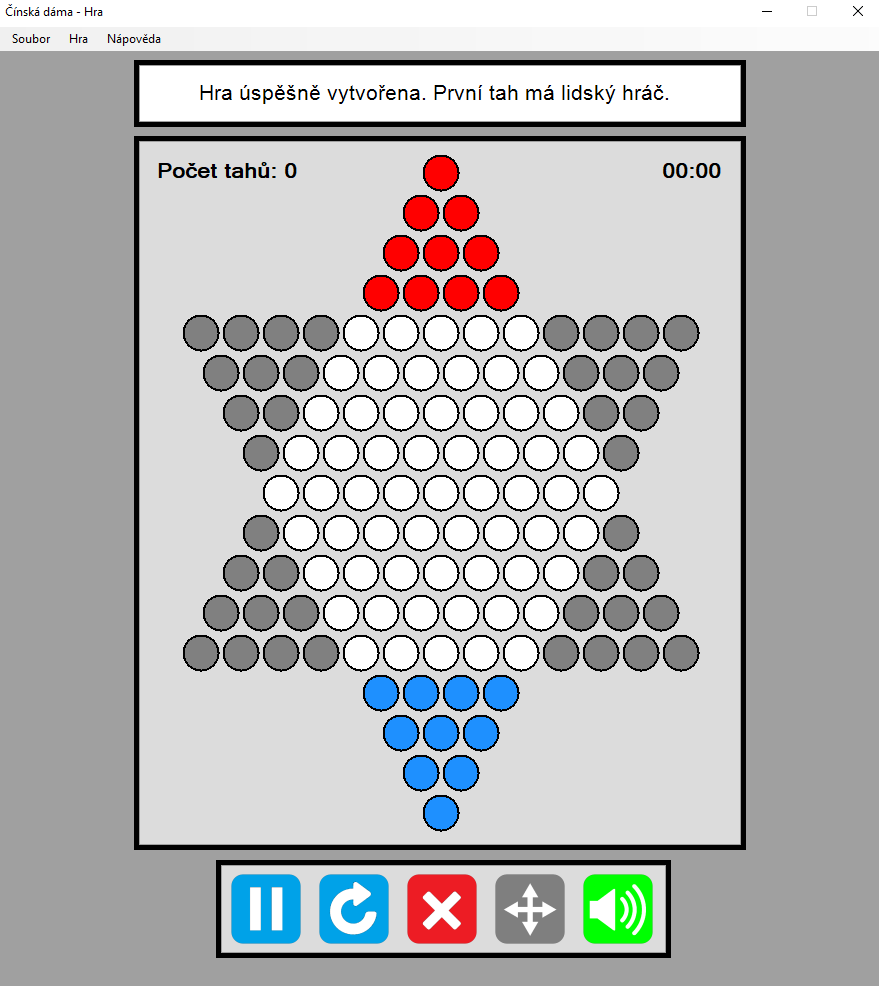
\includegraphics[width=0.7\textwidth]{Figures/HerniOkno.png}
	\caption{Herní okno aplikace}
    \label{fig:HerniOkno}
\end{figure}

Herní okno je tvořeno třemi částmi. Odshora první částí je informační panel, který slouží jako dodatečný prostředek k informování uživatele o průběhu hry. Na obrázku \ref{fig:HerniOkno} obsaženém v této práci informuje uživatele o úspěšném vytvoření hry a prvním hráči na tahu, kromě toho informační panel vypisuje také informace o výsledku her nebo simulací a také během provádění pohybů počítačových hráčů informuje uživatele o tom, pro kterého počítačového hráče je právě vypočítáván tah. Zejména u her s větším množstvím počítačových hráčů vyšších obtížností totiž trvá provedení tahu pro všechny počítačové hráče i několik sekund, a uživatel by mohl nabýt dojmu, že aplikace přestala reagovat. Informační panel také informuje hráče o případném pozastavení hry.

Pod informačním panelem se pak nachází okno zobrazující průběh samotné hry. V aplikaci nese název \lstinline$herniPanel$, a obsahuje dvě naprosto nezbytné události -– událost \lstinline$Paint$, která umožňuje vykreslování jednotlivých objektů, a událost \lstinline$MouseClick$, která reaguje na uživatelova kliknutí myší, což umožní uživateli přesouvání svých kamenů po herní desce. Podrobněji je komunikace mezi herním oknem a hrou popsána v následující podkapitole.

Pro implementaci okna zobrazujícího průběh hry byla nejprve využita třída \lstinline$Panel$. Ta je u~méně rozsáhlých aplikací adekvátním řešením, nicméně u této aplikace se využívá poměrně vysoké množství objektů, a pravděpodobně z tohoto důvodu bylo při hře patrné nepříjemné blikání celé herní desky. Proto je namísto třídy \lstinline$Panel$ využita třída \lstinline$DoubleBufferedPanel$ \cite{doublebuffered}, která z třídy panel dědí. Při využití vlastnosti \lstinline$DoubleBuffered$ překresluje prvek svou plochu pomocí sekundární vyrovnávací paměti, což ve výsledku zabrání blikání.

Mimo to je v tomto okně zobrazena informace o počtu tahů a o uběhlém čase. Vlevo nahoře je vyznačen počet tahů, který je v tomto kontextu chápán jako počet kol, ve kterých všichni hráči táhli, nikoli jako součet počtů tahů všech hráčů. Vpravo nahoře se pak nalézá časomíra, která v~minutách a sekundách měří čas uplynulý od začátku hry. V případě pozastavení hry ze strany uživatele je zastavena také časomíra, spuštěna je souběžně s opětovným spuštěním hry. Oba tyto údaje jsou čistě informativního charakteru, neváže se na ně žádné omezení na způsob maximálního počtu tahů, po kterém je hra automaticky ukončena, nebo maximální možný interval trvání tahu nebo hry, po jehož uplynutí je hráč nějakým způsobem penalizován.

Pod herním panelem se nachází poslední část herního okna, kterou je kontrolní panel. Ten obsahuje pět tlačítek, sloužících ke kontrole hry ze strany lidského hráče. Prvním je tlačítko sloužící k pozastavení hry. Je dvoustavové, a slouží k pozastavení a následnému spuštění hry. Při pozastavení hry nemůže uživatel hýbat svými kameny, a také je zastavena časomíra. Hru může následně spustit stiskem stejného tlačítka. Vzhled tohoto tlačítka v obou stavech je k dispozici na obrázku \ref{fig:PauzaTlacitko}, resp.~\ref{fig:PlayTlacitko}.

\begin{figure}
	\centering
	\subfloat[Pozastavení hry\label{fig:PauzaTlacitko}]
	{
		
\includegraphics[width=0.16\textwidth]{Figures/pause.png}
	}
	\hspace{2em} % make more space
	\subfloat[Spuštění hry\label{fig:PlayTlacitko}]
	{
		
\includegraphics[width=0.16\textwidth]{Figures/play.png}
	}
	\hspace{2em} % make more space
	\subfloat[Restartování hry\label{fig:RestartTlacitko}]
	{
		
\includegraphics[width=0.16\textwidth]{Figures/restart.png}
	}
	\hspace{2em} % make more space
	\subfloat[Ukončení hry\label{fig:KonecTlacitko}]
	{
		
\includegraphics[width=0.16\textwidth]{Figures/ukoncit.png}
	}
	\caption{Tlačítka sloužící k pozastavení, spuštění, restartování a ukončení hry}
	\label{fig:Tlacitka1}
\end{figure}

Dalším tlačítkem nacházejícím se v kontrolním panelu je restartování hry. Toto tlačítko ukončí současnou hru a ihned vytvoří hru novou, parametry přesně odpovídajícími právě ukončené hře. Samozřejmě by se mohlo stát, že uživatel tlačítko stiskne omylem, čímž by nedopatřením přišel o~svou rozehranou hru. Z toho důvodu je restartování hry nutné znovu potvrdit v dialogovém okně, které se po stisknutí tlačítka zobrazí uživateli. Tlačítko je jednostavové a jeho vzhled je k dispozici na obrázku \ref{fig:RestartTlacitko}.

Uprostřed kontrolního panelu se nachází další jednostavové tlačítko, jehož účel je podobný jako v případě tlačítka sloužícího k restartování hry. Toto tlačítko také ukončí hru, ale na rozdíl od předchozího tlačítka nevytvoří novou hru, namísto toho je uživatel vracen zpátky do hlavního menu. Stejně jako u předchozího tlačítka je ale nutné volbu potvrdit v dialogovém okně, protože i u tohoto tlačítka hrozí nechtěné stisknutí tlačítka, které by uživatele připravilo o rozehranou hru. Tlačítko má motiv křížku a je vyobrazeno na obrázku číslo \ref{fig:KonecTlacitko}.

Dále se v tomto panelu nachází tlačítko sloužící k ukončení tahu. To je sice také dvoustavové, stejně jako tlačítko sloužící k pozastavení hry, na rozdíl od něj ale nemá v obou stavech určenou nějakou funkci, aktivní je totiž pouze v jednom z těchto stavů. Tlačítko ukončuje tah, týká se to ale pouze tahů prováděných skoky, nikoli tahů na sousední pole, které jsou ukončovány automaticky. Princip je tedy takový, že uživatel provede první skok, čímž dojde k aktivaci tohoto tlačítka, a po provedení libovolného množství skoků hráč svůj tah ukončí stiskem tlačítka, přičemž se tlačítko opět stává neaktivní. Uživatel nicméně nemusí k ukončení tahu používat toto tlačítko, tah může ukončit také kliknutím na právě posunutý kámen. Vyobrazení tlačítka v obou stavech je na obrázku \ref{fig:KonecTahuDisabled}~a~\ref{fig:KonecTahuEnabled}.

\begin{figure}
	\centering
	\subfloat[Neaktivní\label{fig:KonecTahuDisabled}]
	{
		
\includegraphics[width=0.16\textwidth]{Figures/konecTahuDisabled.png}
	} 
	\hspace{2em} % make more space
	\subfloat[Aktivní, ukončení tahu\label{fig:KonecTahuEnabled}]
	{
		
\includegraphics[width=0.16\textwidth]{Figures/konecTahuEnabled.png}
	}
	\hspace{2em} % make more space
	\subfloat[Přehrávaní zvuků\label{fig:ZvukOn}]
	{
		
\includegraphics[width=0.16\textwidth]{Figures/zvukOn.png}
	} 
	\hspace{2em} % make more space
	\subfloat[Zvuky jsou ztišeny\label{fig:ZvukOff}]
	{
		
\includegraphics[width=0.16\textwidth]{Figures/zvukOff.png}
	}
	\caption{Tlačítka sloužící k ukončení tahu a kontrole přehrávání zvuků}
	\label{fig:Tlacitka2}
\end{figure}

Poslední tlačítko slouží k ovládání zvuků. Přesněji řečeno určuje, jestli při určitých událostech dojde k přehrání daného zvuku nebo ne. Jsou celkem tři události, při kterých může dojít k přehrání zvuku: výběr a přesun kamene, ukončení tahu a konec hry, přičemž v případě výhry, prohry nebo remízy je přehrán odlišný zvuk. Tyto zvuky by ale mohly být některými uživateli považovány na rušivé, proto je zde možnost zvuky stiskem jediného tlačítka vypnout. Uživatel je samozřejmě také může později zapnout, tlačítko je tedy dvoustavové. Vzhled tohoto tlačítka v obou stavech je k~dispozici na obrázku \ref{fig:ZvukOn} a \ref{fig:ZvukOff}.

Kromě zmíněného zahrnuje herní okno také jednoduchý panel nástrojů. Ten umožňuje kontrolu hry nebo aplikace ve srozumitelné, textové podobě. Mimo to umožňuje ovládání aplikace vybranými klávesovými zkratkami. Panel nástrojů zahrnutý v herním okně obsahuje celkem tři nabídky: \textsf{Soubor}, \textsf{Hra} a \textsf{Nápověda}. Možnosti nabízené v každé z nabídek můžeme vidět na obrázku \ref{fig:PanelNastroju}.

\begin{figure}
	\centering
	\subfloat[Nabídka soubor\label{fig:PanelNastrojuSoubor}]
	{
		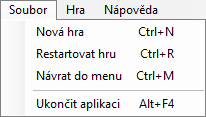
\includegraphics[width=0.3\textwidth]{Figures/PanelNastrojuSoubor.png}
	} 
	\hspace{3em} % make more space
	\subfloat[Nabídka hra\label{fig:PanelNastrojuHra}]
	{
		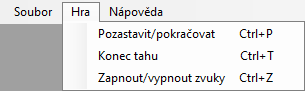
\includegraphics[width=0.45\textwidth]{Figures/PanelNastrojuHra2.png}
	} 
	\hspace{3em} % make more space
	\subfloat[Nabídka nápověda\label{fig:PanelNastrojuNapoveda}]
	{
		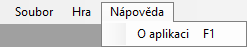
\includegraphics[width=0.4\textwidth]{Figures/PanelNastrojuNapoveda2.png}
	} 
	\caption{Dostupné nabídky panelu nástrojů}
	\label{fig:PanelNastroju}
\end{figure}

Každý hráč má přidělenou vlastní barvu, vzhledem k šesticípému rozložení herní desky je také přidělováno šest různých barev. Občas se ale některé kameny nebo pole od ostatních odlišují. Jeden z těchto případů nastává při zvýraznění kamene, tato situace je na příkladu zvýraznění kamene lidského hráče znázorněna na obrázku číslo \ref{fig:ZvyrazneniHracovaPole}. Ke zvýraznění kamene dochází u lidského a počítačového hráče z odlišných důvodů. U lidského hráče je znázorněn vždy ten kámen, na který uživatel jako poslední klikl. Díky tomuto zvýraznění je tedy uživateli jasné, se kterým kamenem právě manipuluje. U počítačového hráče dochází po konci tahu ke zvýraznění jím přesunutého kamene, díky čemuž je pak uživateli jasné, na jakou pozici se počítačový hráč během tahu posunul. Pro zvýraznění kamenů byly vytvořeny třídy, a to sice \lstinline$ZvyrazneniPoleLidskehoHrace$ a~\lstinline$ZvyrazneniPolePocitacovehoHrace$.

\begin{figure}
	\centering
	
\includegraphics[width=0.3\textwidth]{Figures/ZvyrazneniHracovaPole.png}
	\caption{Zvýraznění hráčova pole}
    \label{fig:ZvyrazneniHracovaPole}
\end{figure}

Kromě nové pozice kamene ale uživatele může zajímat také stará pozice kamene, tedy umístění kamene před provedením tahu. Z toho důvodu bylo potřeba vymyslet nějaký způsob, jakým uživatele informujeme o poloze kamenů před provedením tahu. Jako nejintuitivnější způsob k dosažení tohoto cíle bylo vybráno označení původní polohy kamene bledším odstínem barvy daných hráčů. V aplikaci má toto obarvení pole vlastní objekt, \lstinline$VychoziPolePocitacovehoHrace$, zde můžeme příklad označení původní polohy kamene pro každého počítačového hráče najít na obrázku číslo \ref{fig:VychoziPole}. Pole je tímto způsobem obarveno vždy pouze po dobu jednoho tahu, po provedení dalšího tahu už dané pole tímto způsobem označeno není.

\begin{figure}
	\centering
	\subfloat[Červený\label{fig:VychoziPoleCerveny}]
	{
		
\includegraphics[width=0.15\textwidth]{Figures/VychoziPoleCerveny.png}
	} 
	\hspace{1em} % make more space
	\subfloat[Zelený\label{fig:VychoziPoleZeleny}]
	{
		
\includegraphics[width=0.15\textwidth]{Figures/VychoziPoleZeleny.png}
	}
		\hspace{1em} % make more space
	\subfloat[Fialový\label{fig:VychoziPoleFialovy}]
	{
		
\includegraphics[width=0.15\textwidth]{Figures/VychoziPoleFialovy.png}
	}
		\hspace{1em} % make more space
	\subfloat[Hnědý\label{fig:VychoziPoleHnedy}]
	{
		
\includegraphics[width=0.15\textwidth]{Figures/VychoziPoleHnedy.png}
	}
		\hspace{1em} % make more space
	\subfloat[Žlutý\label{fig:VychoziPoleZluty}]
	{
		
\includegraphics[width=0.15\textwidth]{Figures/VychoziPoleZluty.png}
	}
	\caption{Vyznačení původní polohy kamene pro jednotlivé počítačové hráče}
	\label{fig:VychoziPole}
\end{figure}

\section{Komunikace mezi herním oknem a hrou}
Jak už bylo zmíněno v předchozí podkapitole, k vykreslování celé herní desky se všemi objekty dochází v metodě \lstinline$Paint$ prvku \lstinline$herniPanel$. Tuto metodu můžeme nalézt v třídě \lstinline$HraForm$. Samotná hra je ale vytvářena a spravována v jiné třídě, a to ve třídě \lstinline$Hra$. Je tedy nutné nějakým způsobem dostat údaje o aktuálním stavu hry ze třídy \lstinline$Hra$ do třídy \lstinline$HraForm$. Pro tyto účely je ve třídě \lstinline$Hra$ implementována klíčová metoda \lstinline$HerniPrvky$, jejíž návratovou hodnotou jsou kolekce všech objektů vyobrazovaných na herní desce (implementace této metody je znázorněna na výpisu \ref{src:metodaHerniPrvky}).

\begin{lstlisting}[label=src:metodaHerniPrvky,caption={Metoda vracející kolekce všech vyobrazovaných objektů}]
public (List<Pole>, List<LidskyHrac>, List<PocitacovyHrac>, List<MoznyTahLidskehoHrace>, ZvyrazneniPoleLidskehoHrace, List<ZvyrazneniPolePocitacovehoHrace>, List<VychoziPolePocitacovehoHrace>) HerniPrvky()
{
    return (herniPole, poleLidskehoHrace, polePocitacovehoHrace, mozneTahyLidskehoHrace, zvyrazneniPoleLidskehoHrace, zvyraznenaPolePocitacovehoHrace, vychoziPolePocitacovehoHrace);
}
\end{lstlisting}

V tuto chvíli máme sice ve třídě \lstinline$HraForm$ veškeré kolekce potřebné k vyobrazení celé herní desky, neznáme ale zatím žádný způsob, který by mohl být použit k vykreslení jednotlivých objektů. Z toho důvodu obsahuje každý objekt, který budeme chtít vykreslovat, metodu umožňující kreslení. Názorný příklad si ukážeme na kamenu lidského hráče. Jedním z argumentů události \lstinline$Paint$ prvku \lstinline$herniPanel$ je \lstinline$PaintEventArgs$ \cite{painteventargs}, což je třída sloužící k poskytování dat události \lstinline$Paint$. K vykreslení jednotlivých objektů pak stačí v daných objektech implementovat metodu, které předáme instanci třídy \lstinline$PaintEventArgs$. U kamene lidského hráče má tato metoda jméno \lstinline$NakresliLidskehoHrace$, přičemž v této metodě stačí pak využít instanci třídy ke kreslení a nakreslit útvar, s tím že barva a poloha tohoto útvaru závisí na parametrech daného objektu. V metodě \lstinline$Paint$ pak už jen stačí projít v cyklu všechny kolekce objektů získané pomocí metody \lstinline$HerniPrvky$, zavolat u všech objektů metody určené pro jejich vykreslování, a herní deska je z grafického hlediska hotová.

Pro lepší pochopení jsou ve výpisech \ref{src:metodaNakresliLidskehoHrace} a \ref{src:metodaIteraceKamenyHrace} obsaženy zmíněné metody a postupy.

\begin{lstlisting}[label=src:metodaNakresliLidskehoHrace,caption={Metoda vykreslující kámen lidského hráče}]
public void NakresliLidskehoHrace(PaintEventArgs e)
{
    e.Graphics.FillEllipse(br, this.poz_X_LHr, this.poz_Y_LHr, this.sirkaPole, this.vyskaPole);
    e.Graphics.DrawEllipse(pen, this.poz_X_LHr, this.poz_Y_LHr, this.sirkaPole, this.vyskaPole);
}
\end{lstlisting}

\newpage

\begin{lstlisting}[label=src:metodaIteraceKamenyHrace,caption={Metoda vykreslující postupně všechny kameny lidského hráče}]
foreach (LidskyHrac h in poleLidskehoHrace)
{
    h.NakresliLidskehoHrace(e);
}
\end{lstlisting}

Implementací těchto metod můžeme vykreslování herní desky považovat za vyřešené. Je ale ještě nutné vyřešit uživatelský vstup, tedy přesuny hráčových polí. Ve třídě \lstinline$HraForm$ zajišťuje zpracování uživatelského vstupu událost \lstinline$MouseClick$ prvku \lstinline$herniPanel$, která je vyvolána při každém kliknutí na panel. Z této metody pak voláme metodu \lstinline$PanelKliknuti$ třídy \lstinline$Hra$, které předáme přesné souřadnice uživatelova kliknutí. 

V této metodě je nejprve ověřeno, jestli uživatel vůbec klikl na nějaké herní pole. Pokud ano, je ověřeno, jestli se jedná o některý z jeho kamenů nebo možných tahů. Po ověření následuje provedení příslušného postupu, tyto postupy jsou detailněji popsány v podkapitole \ref{sec:VytvoreniMoznychTahu}. Po vykonání metody \lstinline$PanelKliknuti$ je potřeba uživatelovi zobrazit nový stav herní desky, proto je herní panel obnoven zavoláním metody \lstinline$Refresh$.


\section{Ostatní okna}
Aplikace obsahuje kromě herního okna několik dalších, převážně pomocných oken. Prvním oknem, které se uživateli zobrazí po spuštění aplikace, je hlavní menu (v aplikaci pod názvem \lstinline$MenuForm$, v~této práci obrázek číslo \ref{fig:HlavniMenu}). Kromě zobrazení banneru slouží ke snadnému a přímému přístupu ke všem částem aplikace.

Nyní projdeme zbývající okna postupně v pořadí, v jakém je tlačítko sloužící k jejich otevření umístěno v hlavním menu. Po kliknutí na tlačítko \textsf{Nová hra} je otevřeno okno ve kterém uživatel nastavuje parametry hry (v aplikaci pod názvem \lstinline$ParametryHryForm$, v této práci obrázek číslo \ref{fig:ParametryHry}). V tomto okně si uživatel navolí počet počítačových hráčů, proti kterým bude hrát, jejich obtížnost, a také kdo bude první na tahu. Jediným omezením je, že uživatel musí vždy vybrat některou z~nabízených možností, pokud se pokusí vytvořit hru bez nastavení počtu hráčů nebo začínajícího hráče, je mu zobrazeno dialogové okno s chybovou hláškou.

\begin{figure}
	\centering
	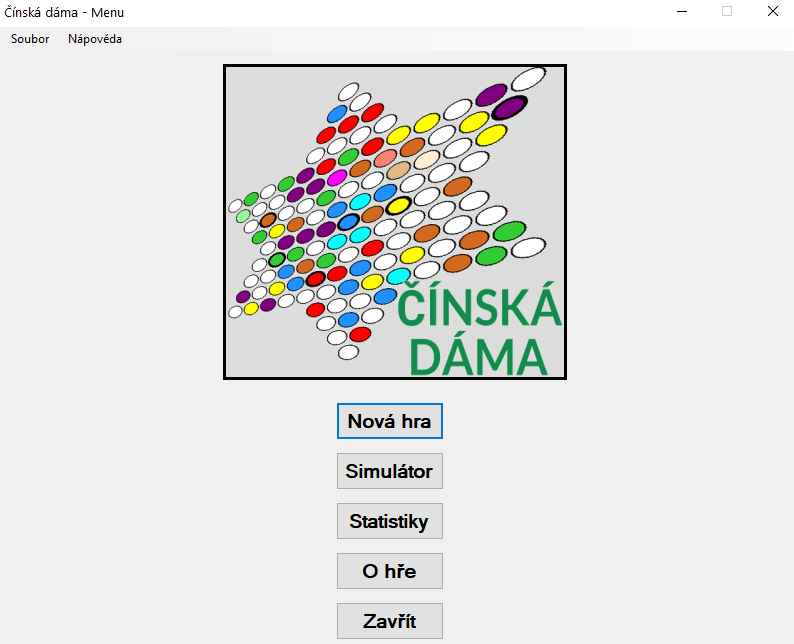
\includegraphics[width=0.6\textwidth]{Figures/HlavniMenu.png}
	\caption{Okno \textsf{Hlavní menu}}
    \label{fig:HlavniMenu}
\end{figure}

\begin{figure}
	\centering
	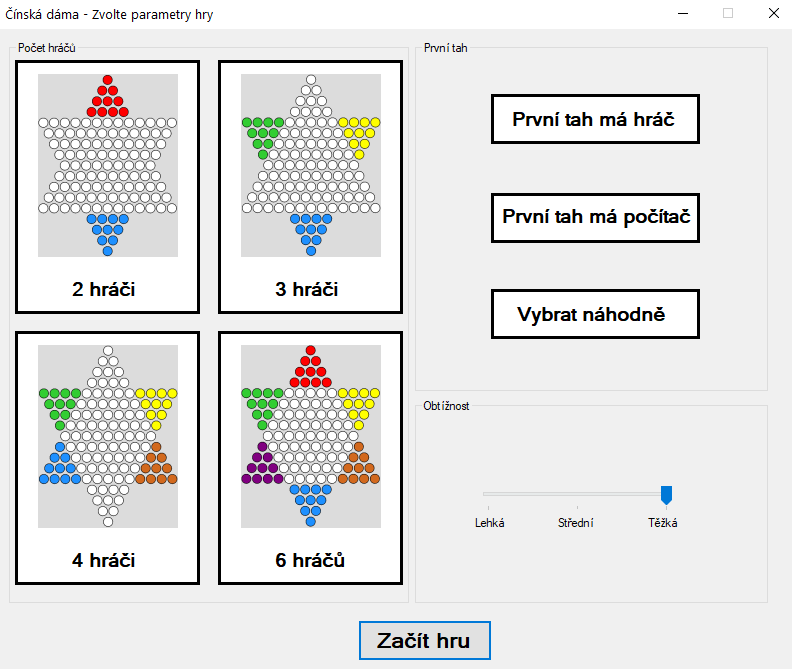
\includegraphics[width=0.6\textwidth]{Figures/ParametryHry.png}
	\caption{Okno \textsf{Parametry hry}}
    \label{fig:ParametryHry}
\end{figure}

Na stejném principu funguje i další okno, které se zobrazí po kliknutí na tlačítko \textsf{Simulátor}. Jedná se o okno, ve kterém uživatel nastavuje parametry simulátoru (v aplikaci pod názvem \lstinline$ParametrySimulatoruForm$, v této práci obrázek číslo \ref{fig:ParametrySimulatoru}). Hráč zde před spuštěním simulace zvolí počet počítačových hráčů hrajících v dané simulaci a také jejich obtížnost. Okno je navrženo s ohledem na co největší srozumitelnost, po výběru určitého počtu hráčů je vždy zobrazena herní deska s odpovídajícím rozvržením k danému počtu hráčů, a obtížnosti jednotlivých hráčů jsou umístěny na místech, kde by se nacházeli skuteční hráči při hře s využitím fyzické desky.

\begin{figure}
	\centering
	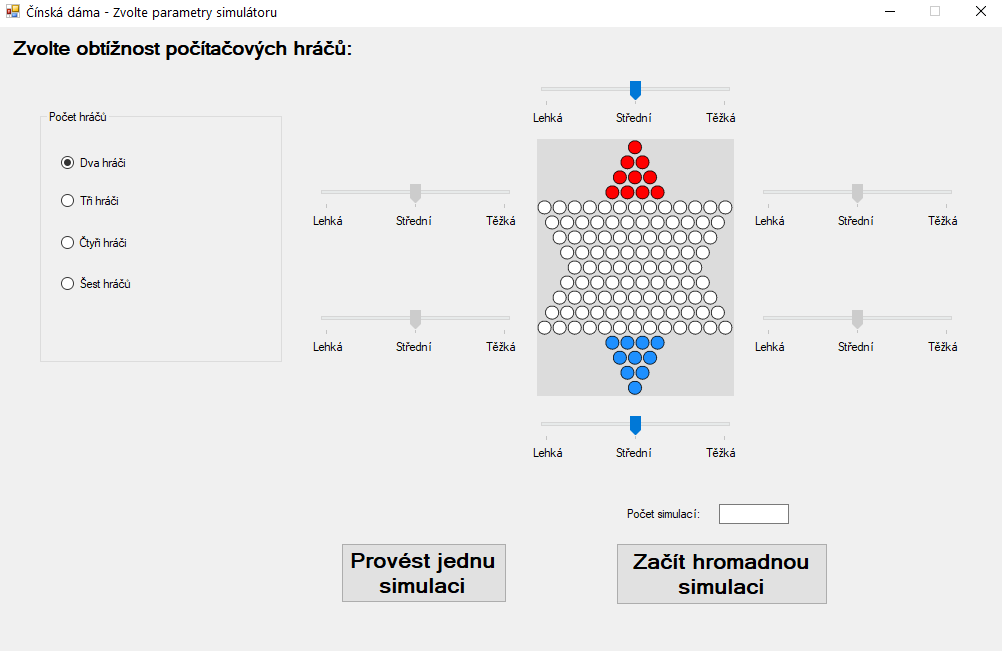
\includegraphics[width=0.6\textwidth]{Figures/ParametrySimulatoru.png}
	\caption{Okno \textsf{Parametry simulátoru}}
    \label{fig:ParametrySimulatoru}
\end{figure}
Dalším oknem nacházejícím se v aplikaci je okno se statistikami (v aplikaci jej najdeme pod názvem \lstinline$StatistikyForm$, v této práci obrázek číslo \ref{fig:Statistiky}). Jeho účelem je poskytnutí uživatelsky srozumitelné interpretace souboru \textsf{Statistiky.txt}, který obsahuje záznamy o všech provedených simulacích. Jak napovídá text uvedený v samotném okně, okno neslouží k zaznamenávání her lidského hráče. zaznamenávány jsou zde pouze výsledky simulací.

\begin{figure}
	\centering
	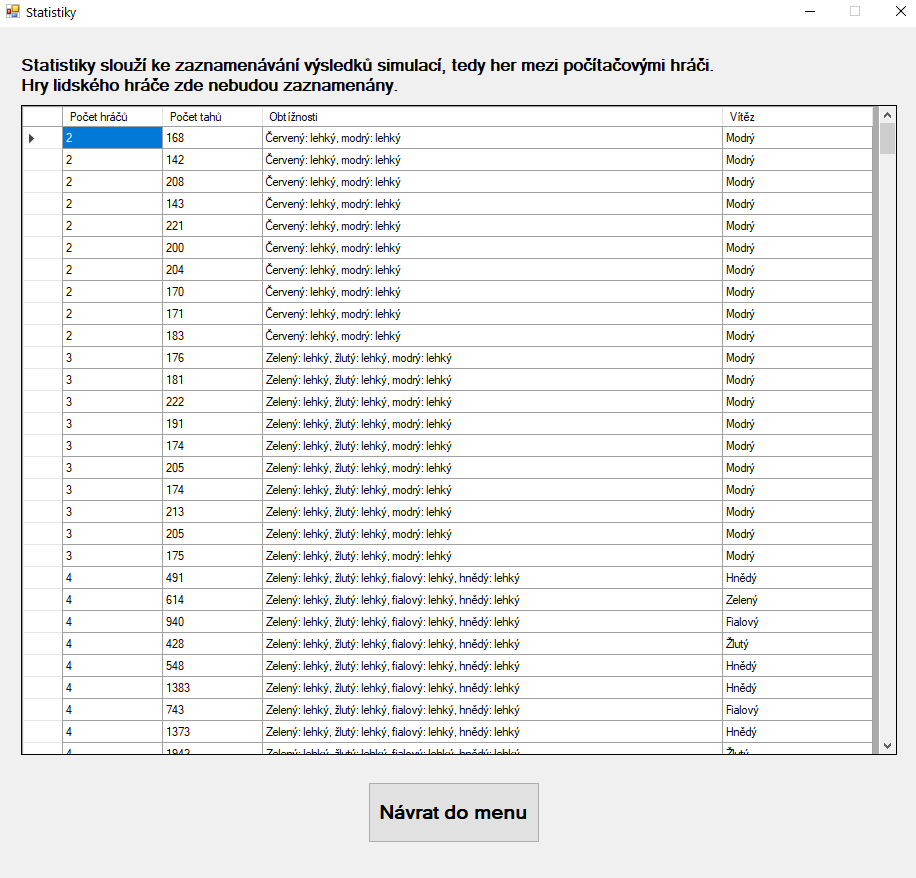
\includegraphics[width=0.6\textwidth]{Figures/Statistiky.png}
	\caption{Okno \textsf{Statistiky}}
    \label{fig:Statistiky}
\end{figure}

Posledním oknem je okno \textsf{O hře} (v aplikaci pod názvem \lstinline$InformaceForm$, v této práci obrázek číslo \ref{fig:OHre}). Otevřít jej lze dvěma způsoby. Jednak po výběru možnosti \textsf{O hře} v hlavním menu, a~jednak po výběru možnosti \textsf{Nápověda}, která je k dispozici v panelu nástrojů při hře. Okno obsahuje základní informace týkající se pravidel a ovládání hry, které by mohly novému uživateli pomoci v~pochopení hry. Kromě toho je zde také krátká zmínka o autorovi aplikace a o účelu jejího vytvoření.

\begin{figure}
	\centering
	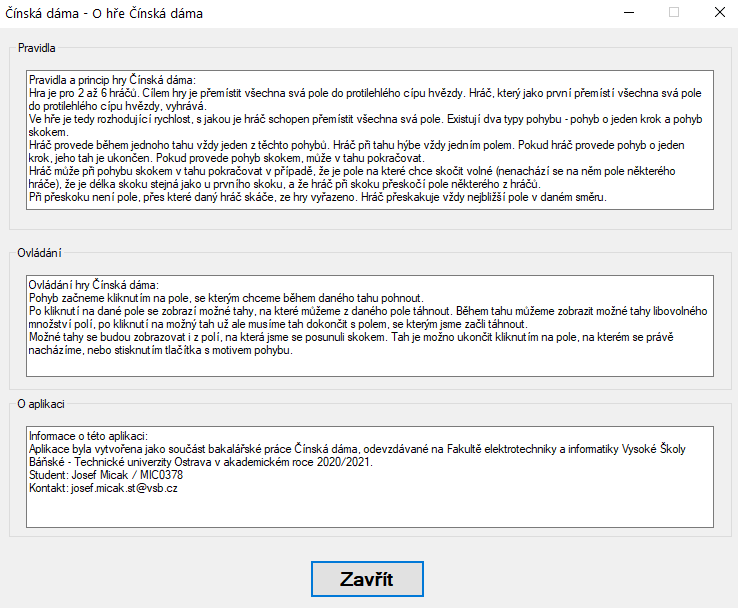
\includegraphics[width=0.6\textwidth]{Figures/OHre.png}
	\caption{Okno \textsf{O hře}}
    \label{fig:OHre}
\end{figure}
\endinput